%%%%%%%%%%%%%%%%%%%%%%%%%%%%%%%%%%%%%%%%%
% Journal Article
% LaTeX Template
% Version 1.3 (9/9/13)
%
% This template has been downloaded from:
% http://www.LaTeXTemplates.com
%
% Slightly updated by  Marc Uetz
%
% Original author:
% Frits Wenneker (http://www.howtotex.com)
%
% License:
% CC BY-NC-SA 3.0 (http://creativecommons.org/licenses/by-nc-sa/3.0/)
%
%%%%%%%%%%%%%%%%%%%%%%%%%%%%%%%%%%%%%%%%%

%----------------------------------------------------------------------------------------
%	PACKAGES AND OTHER DOCUMENT CONFIGURATIONS
%----------------------------------------------------------------------------------------

\documentclass[twoside]{article}

\usepackage{lipsum} % Package to generate dummy text throughout this template
\usepackage{amsmath,amssymb,amsthm,appendix,graphicx} % Mathematical Symbols, styles, etc

\newtheorem{theorem}{Theorem}[section]
\newtheorem{lemma}[theorem]{Lemma}
\newtheorem{proposition}[theorem]{Proposition}
\newtheorem{corollary}[theorem]{Corollary}
\newtheorem{definition}{Definition}[section]


\usepackage[sc]{mathpazo} % Use the Palatino font
\usepackage[T1]{fontenc} % Use 8-bit encoding that has 256 glyphs
\linespread{1.05} % Line spacing - Palatino needs more space between lines
\usepackage{microtype} % Slightly tweak font spacing for aesthetics
\usepackage[utf8]{inputenc}

\usepackage[hmarginratio=1:1,top=32mm,columnsep=20pt]{geometry} % Document margins
\usepackage{multicol} % Used for the two-column layout of the document
\usepackage[hang, small,labelfont=bf,up,textfont=it,up]{caption} % Custom captions under/above floats in tables or figures
\usepackage{booktabs} % Horizontal rules in tables
\usepackage{float} % Required for tables and figures in the multi-column environment - they need to be placed in specific locations with the [H] (e.g. \begin{table}[H])
\usepackage{hyperref} % For hyperlinks in the PDF
\usepackage[dutch]{babel}
\usepackage{lettrine} % The lettrine is the first enlarged letter at the beginning of the text
\usepackage{paralist} % Used for the compactitem environment which makes bullet points with less space between them
\usepackage{algorithmicx}
\usepackage[]{algorithm2e}
\usepackage{algpseudocode}
\usepackage{pifont}
\usepackage{abstract} % Allows abstract customization
\renewcommand{\abstractnamefont}{\normalfont\bfseries} % Set the "Abstract" text to bold
\renewcommand{\abstracttextfont}{\normalfont\small\itshape} % Set the abstract itself to small italic text

\usepackage{titlesec} % Allows customization of titles
%\renewcommand\thesection{\Roman{section}} % Roman numerals for the sections
%\renewcommand\thesubsection{\Roman{subsection}} % Roman numerals for subsections
\titleformat{\section}[block]{\large\scshape}{\thesection.}{1em}{} % Change the look of the section titles
\titleformat{\subsection}[block]{\large}{\thesubsection.}{1em}{} % Change the look of the section titles

\usepackage{fancyhdr} % Headers and footers
\pagestyle{fancy} % All pages have headers and footers
\fancyhead{} % Blank out the default header
\fancyfoot{} % Blank out the default footer
\fancyhead[C]{C.H.M.\ van den Bogaard, D.T.R. Ikink, F.\ Seuren, R.\ Monshouwer: \shorttitle} % Custom header text
\fancyfoot[RO,LE]{\thepage} % Custom footer text

%----------------------------------------------------------------------------------------
%	TITLE SECTION
%----------------------------------------------------------------------------------------

\newcommand{\articletitle}{Fast partition refinement, a Python implementation}
\newcommand{\shorttitle}{Python fast partitioning}

\title{\vspace{-15mm}\fontsize{24pt}{10pt}\selectfont\textbf{\articletitle}} % Article title

\author{
\large
\textsc{Christiaan van den Bogaard, Dion Ikink, Fleur Seuren, and Rogier Monshouwer}\thanks{Thanks to our helpful mentor.}\\[2mm] % Your name
\normalsize University of Twente \\ % Your institution
\normalsize \href{mailto:c.h.m.vandenbogaard@student.utwente.nl}{c.h.m.vandenbogaard@student.utwente.nl},
\href{mailto:d.t.r.ikink@student.utwente.nl}{d.t.r.ikink@student.utwente.nl} \\
\normalsize\href{mailto:f.seuren@student.utwente.nl}{f.seuren@student.utwente.nl}, % Your email addresses
\href{mailto:r.monshouwer@student.utwente.nl}{r.monshouwer@student.utwente.nl}
}

\date{\today}

%----------------------------------------------------------------------------------------

\begin{document}

\thispagestyle{empty}
\maketitle % Insert title

%----------------------------------------------------------------------------------------
%	ABSTRACT
%----------------------------------------------------------------------------------------

\begin{abstract}

Graaf isomorfisme is een probleem dat wiskundigen al lang bezig houdt, want er is nog steeds geen algoritme gevonden dat het probleem efficiënt oplost. Het doel van ons onderzoek was het vinden en implementeren van een correct en zo efficiënt mogelijk algoritme om isomorfisme tussen grafen aan te tonen. De keuze is gevallen op het algoritme van Hopcroft, dat oorspronkelijk gebruikt werd voor DFA minimalisatie. Niet alleen hebben we dit algoritme geïmplementeerd, we hebben ook geprobeerd aan te tonen dat het algoritme een tijdscomplexiteit van orde $O(m\log_{2}(n))$ heeft. Dat laatste bleek lastiger dan we verwachtten, maar de implementatie is meerdere malen sneller dan veel andere algoritmes. Uiteraard is er ruimte voor verbetering, maar het doel van het onderzoek is bereikt: we hebben een snel en efficiënt algoritme in Python geschreven. Verdere toelichting wat betreft de implementatie en de onderzoeksresultaten vindt u in de rest van deze paper.

\end{abstract}

%----------------------------------------------------------------------------------------
%	ARTICLE CONTENTS
%----------------------------------------------------------------------------------------

\begin{multicols}{2} % Two-column layout throughout the main article text



%------------------------------------------------
\section*{Inleiding}
\begin{quote}
\textit{''Gegeven twee eindige grafen $G$ en $H$, bestaat er een isomorfisme tussen $G$ en $H$?''}
\end{quote}

Het bovenstaande probleem staat bekend als het graaf isomorfisme probleem  (GI), één van de meest bestudeerde onderwerpen binnen de discrete wiskunde en theoretische informatica. Een isomorfisme tussen twee grafen vinden is op zich geen moeilijk probleem. Een oplossing zou kunnen zijn om van allee bijectieve functies van $G$ naar $H$ te controleren of deze een isomorfisme defini\"eren. Het probleem van deze oplossing is dat dit enorm veel tijd kost. Als je bijvoorbeeld voor twee grafen met 10 punten elke seconde \'e\'en bijectie zou onderzoeken ben je al 42 dagen bezig. Niet heel erg snel dus. Daarom is het echte probleem een algoritme te bedenken dat tussen twee willekeurige grafen effici\"ent kan beslissen of deze issomorf of niet isomorf zijn. Voor verschillende klassen van grafen is er inderdaad een algoritme gevonden maar hoewel er honderden onderzoeken over zijn gepubliceerd, is er nog altijd geen oplossing gevonden die toepasbaar is op alle mogelijke grafen. Niet voor niets bevindt de complexiteit van dit probleem zich in een geheel nieuwe complexiteitsklasse, tussen de problemen die oplosbaar zijn in polynomiale tijd (P) en de beslisproblemen wiens oplossingen verifieerbaar zijn in polynomiale tijd (NP-complete).

Een van de bestaande technieken die veel gebruikt wordt om het GI probleem op te lossen is ''partition refinement''. In dit artikel wordt het idee achter ''partition refinement'' uitgelegd. Daarnaast wordt er een zeer effici\"ente Python implementatie van deze techniek gegeven. Dit algoritme, dat gebaseerd is op een door Hopcroft~\cite{MR0403320} bedacht algoritme voor het minimaliseren van DFA's heeft namelijk een complexiteitklasse van $O(m \log_{2} (n)$ met $m= \text{aantal lijnen}$ en $n = \text{aantal punten}$, terwijl een standaard implementatie maar een tijdscomplexiteitsklasse van $O(n^2)$ heeft.

%------------------------------------------------
\section{Theoretische onderbouwing}
In deze sectie wordt de theorie achter zowel ''partition refinement'' als het algoritme van Hopcroft uitgelegd.

\subsection{Partition refinement}
Het idee achter partition refinement is dat een isomorfisme de omgeving (de verzameling buren) van een punt $v$ in stand houdt. Punt $v$ in graaf $G$ heeft dus dezelfde omgeving als zijn afbeelding $\phi(v)$ in H. Hieruit volgt dat de graad van $v$ gelijk is aan de graad van $\phi(v)$. Er kan dus een initi\"ele partitie gemaakt worden op basis van graad. In dit artikel betekent de kleuring van een graaf hetzelfde als de partionering van een graaf. Door een partitie een kleur toe te wijzen kunnen we makkelijke illustreren hoe de graaf wordt verdeeld.

Omdat alle punten nu een bepaalde kleur hebben kan deze initi\"ele partitie verfijnd worden, namelijk op basis van de kleuromgeving van punt $v$. Deze kleuromgeving is als volgt gedefinieerd:

\begin{definition}
Neem $\alpha$, een partitie van graaf $G$ met $k$ verschillende kleuren en  $\alpha^{c}$ de verzameling punten van $G$ met kleur $c \in \{1,\ldots,k\}$. Twee punten $u,v \in V(G)$ hebben een \textbf{verschillende kleuromgeving} als er een kleur $c \in \{1,\ldots,k\}$ is zodanig dat $|N(u)\cap\alpha^{c}| \neq |N(v)\cap\alpha^{c}|$. Als dit niet geldt hebben de twee punten een \textbf{gelijke kleuromgeving}
\cite{slides_DFA}
\end{definition}


De partitie wordt nu dus verfijnd door elke groep op te splitsen in punten met een verschillende kleuromgeving, waarbij elke nieuwe groep uiteraard weer een nieuwe kleur krijgt. Omdat er weer punten met nieuwe kleuren zijn bijgekomen kan ook deze partitie weer verfijnd worden op basis van kleuromgeving. Dit proces wordt herhaald tot het niet meer mogelijk is om een groep op te splitsen in nieuwe groepen met verschillende kleuromgevingen. Op dat moment bevinden zich in elke groep alleen maar elementen met dezelfde kleuromgeving, er wordt dan gesproken van een stabiele partitie.

Zoals eerder vermeld was behoudt een isomorfisme de omgeving van een bepaald punt, een isomorfisme behoudt dus ook de kleuromgeving van een bepaald punt. In twee isomorfe grafen bevindt zich dus een gelijke stabiele partitie. Met behulp van zo'n stabiele partitie kan een van deze drie situaties ontstaan.
\begin{enumerate}
\item Er kan een isomorfisme gedefinieerd worden.
\item Er bestaat geen isomorfisme en er wordt geconcludeerd dat  de twee grafen niet isomorf zijn.
\item Het kan zijn dat er het nog geen bijectie ontstaat en het dus nog niet zeker is of er een isomorfisme is.
\end{enumerate}

\subsection{Hopcrofts algoritme}
Het nadeel van bovenstaand algoritme is dat het, hoewel het een enorme verbetering is ten opzichte van een brute force methode, nog steeds een complexiteit van $O(n^2)$ heeft, wat het nog steeds niet efficiënt genoeg maakt. Daarom is er gezocht naar een snellere implementatie van dit algoritme, zoals het algoritme van Hopcroft. Er wordt dus nog steeds gezocht naar een stabiele partitie $\alpha$ voor graaf $G$ alleen we proberen om de tijdcomplexiteit van de verfijningsoperatie zo klein mogelijk te maken. We maken hierbij gebruik van de volgende verfijning:

\begin{lemma}
Neem C een kleurgroep in de huidige partitie $\alpha$ en definieer voor alle $i \geq 0$ $D_{i}$ als het aantal punten met precies $i$ buren in $C$. Door elke kleurgroep $C' \neq C$ in de huidige partitie te vervangen door de niet-lege kleurgroepen $C'_{i} := C'\cap D_{i}$ wordt de ruwste stabiele partitie voor graaf $G$ gevonden.
\cite{slides_DFA}
\label{verfijn}
\end{lemma}

De verfijning die hierboven beschreven staat kan ge\"implementeerd worden met een complexiteitsklasse van $O(|E^{-}(C)|)$. Dat komt omdat bij iedere iteratie van het algoritme het niet nodig is om de punten in alle overige kleurklassen te checken.

\begin{lemma}
Stel $C \subseteq V(G)$ wordt tijdens een iteratie gesplitst in $C_{0}, \ldots, C_{k}$. Dan geldt $\forall a \in \{0,\ldots,k\}$: als partitie $\alpha$ stabiel is voor $C$ en voor $C_{b}$ $\forall b \in \{0,\ldots,k\}/\{a\}$, dan is partitie $\alpha$ ook stabiel voor $C_{a}$.
\label{weglaat}
\end{lemma}

\begin{proof}
Stel $\alpha$ is niet stabiel voor $C_{a}$:\\
Dan: $ u,v \in V(G)$ met $u \equiv_{\pi} v$ zodanig dat $u \in C_{a}$ en $v \not \in C_{a}$.\\
Omdat partitie $\alpha$ stabiel was voor $C$ geldt: $u,v \in C$.\\
Omdat $C_{0},\ldots,C_{a},\ldots,C{k}$ een partitie is van $C$ geldt: $\exists b \neq a $ zodanig dat $v \in C_{a}$ en $u \not \in C_{a}$.\\
Dan geldt: $\alpha$ is niet stabiel voor $C_{b}$, een tegenstelling.
\cite{slides_DFA}
\end{proof}

Het is dus niet nodig om de partitie te verfijnen voor alle kleurklassen, waardoor het mogelijk is de verfijningsstap voor $C$ te implementeren met een tijd complexiteit van $O(|E^{-}(C)|)$, lineair over alle punten die buren hebben in $C$. In de volgende sectie zal de Python implementatie voor een algoritme beschreven worden en bewezen worden dat deze een complexiteitsklasse van $O(|E^{-}(C)|)$ heeft.

%------------------------------------------------

\section{Implementatie}
Het algoritme hieronder staat beschreven in pseudocode, maar het wordt kort toegelicht.

We beginnen door alle punten $v_i$ in te delen in een partitie $C_j$ op basis van degree. Vervolgens vullen we een queue ($Q$) met alle partities.
Zolang $Q$ niet leeg is, verfijnen we de eerste partitie $C$ in $Q$, op de manier beschreven in lemma \ref{verfijn} en verwijderen deze uit de queue.

We splitsen dus de partities $ C' $  in nieuwe partities op basis van hoeveel buren hun punten in $C$ hebben. Dit doen we door voor alle $v_{i}$ in $C$ te bij te houden welke buren $N(v_{i})$ ze hebben. Bijvoorbeeld, als $v_{i}$ in $C$ een buur $v_{x}$ in een bepaalde partitie $C'$ heeft, dan stijgt de $neighbour\_count$ van die vertex met 1. Nadat over alle $v_{i} \in C$ geïtereerd is weten we dus voor alle $v \not \in  C$ hoeveel buren deze in $C$ hebben.

Vervolgens worden van al deze punten groepen $d\_count$ gemaakt op basis van dit aantal buren in $C$. $d\_count(0)$ is bijvoorbeeld de verzameling vertices in $C'$ zonder buren in $C$. Daarna wordt de verfijning toegepast en wordt $C'$ vervangen door de doorsnede van $C'$ met alle verschillende groepen $d\_count$.

Zodra er dus een verschil zit tussen $C'$ en $d\_count(i) | i\geq 0$, wordt dit een nieuwe partitie bij die $neighbour\_count$. Deze nieuwe partities worden op hun beurt weer in de $Q$ gezet. De partitie met de meeste vertices wordt niet in $Q$ gezet, aangezien volgens lemma \ref{weglaat} die partitie stabiel is als alle andere partities ook stabiel zijn.

%------------------------------------------------
\subsection{Bewijs}

We gaan hier bewijzen dat de tijdscomplexiteit van onze implementatie van het verfijningsalgoritme ($generate\_dcounts$) gelijk is aan $ O(|E^{-}(C)|)$,  waar $ E{-}(C) $ het aantal lijnen is dat incident is met punten uit $C$.

\begin{lemma}
De complexiteit van\\ $generate\_dcounts(C)$ van een graaf is $O(|E^{-}(C)|) $,  waarbij  $E^{-}(C)$ het aantal lijnen incident met vertices in $C$.
\end{lemma}

\begin{proof}
De operatie $generate\_dcounts(C) $ kan gezien worden als twee for-loops, de eerste for-loop, itereert voor alle $v$ in $C$ over alle $v'$ in $N(V)$, dus over alle lijnen die incident zijn met die $v$ uit $C$. Dus als je daarna ook over alle $v$ in $C$ itereert, itereer je in totaal over alle lijnen die incident zijn met $C$, $E^{-}(C)$. Elk van deze iteraties is constant $O(1)$ want optellen en doorsnede nemen zijn constante operaties. De orde van de eerste for-loop is dus $O(|E^{-}(C)|)$

Bij de tweede for-loop itereer je nogmaals over alle buren van alle punten in $C$. En ook de operatie binnen al deze iteraties is constant, aangezien het nemen van de vereniging constant is, de orde van de tweede for-loop is dus ook $O(|E^{-}(C)|)$.

De orde van de totale operatie is dus $O(|E^{-}(C)|)$
\end{proof}


%------------------------------------------------
\section{Berekende resultaten}

Voor verschillende grafen en verschillende grootten van grafen hebben wij gekeken hoe lang het duurt voordat van een bepaalde graaf een stabiele partitie is gemaakt. Wij hebben hiervoor twee algoritmes gebruikt, het ene algortime, Refine, was onze implementatie zonder fast partition refinement en het tweede algoritme, Fast Refine, met fast partition refinement.

De resultaten van de metingen zijn gegeven in Appendix~\ref{AppendixA}.

Om toeval uit te sluiten zijn alle tests tien keer uitgevoerd voor beide algoritmes. De gemeten tijden zijn de gemiddelden van de tien uitgevoerde tests. In de laatste kolom is het verschil in uitvoertijd opgenomen, weergegeven als percentages. Een percentage van $100\%$ betekent dat het Fast Refine-algoritme (FR) tweemaal zo snel was als het Refine-algoritme (R) bij het uitvoeren van de test (een verbetering van $100$\% ten opzichte van Refine).

De 'threepaths' grafen, zie figuur \ref{paths} zijn complexe problemen voor het standaard partition refinment algoritme om op te lossen. Ze bevatten lange paden en in elk pad kunnen er maximaal twee vertices van kleur veranderen. In graaf 1 is de partitie na de eerste stap van het algoritme gegeven. Graaf 2 is het resultaat van de volgende iteratie. Aangezien vertices B en F nu veranderd zijn, moeten alle vertices daartussen (C, D en E) ook opnieuw bekeken worden. Zoals hier te zien is kan het algoritme per iteratie maar voor twee vertices in een pad de coloring verfijnen. Graaf 3 geeft de stabiele coloring weer. R heeft dus zeer veel tijd nodig heeft om tot een stabiele partitie te komen. FR pakt het probleem zoals verwacht veel effici\"enter aan. Voor een van de grotere grafen (threepaths5120) is FR ruim 25 keer sneller.

\begin{figure}[H]
\centering
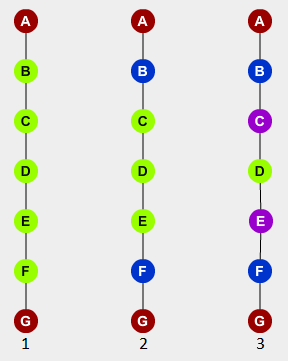
\includegraphics[]{paths.png}
\caption{Schematische weergave van het partitioneren van een pad}
\label{paths}
\end{figure}


%------------------------------------------------
\section{Conclusie}
Het blijkt dus dat Hopcrofts algoritme een slimme manier is om een graaf te partitioneren. Het grote graaf isomorfisme probleem blijkt een lastige opgave te zijn en partition refinement is de veelzijdige hamer in de gereedschapskist om het graaf isomorfisme op te lossen. Het helpt de graaf te onderscheiden in verschillende partities waardoor een bijectie kan ontstaan. John Hopcrofts idee achter DFA minimalisatie bleek een perfecte oplossing om zo snel mogelijk een graaf te partitioneren. Door de grootste partitie niet verder te bezoeken onstaat er een logaritmische partionering waar alleen het zoeken naar de verschillende partities een linear complexiteit heeft. Dit is een hele verbetering ten opzichte van het standaard refine algoritme. Door beide algoritmes te implementeren in Python konden we het volgende concluderen:

\begin{enumerate}
\item Onze implementatie bewijst dat het mogelijk is om Hopcrofts algoritme te implementeren in de tijdscomplexiteitsklasse van orde $O(m\log_{2}(n))$ door te bewijzen dat ``Refine`` in lineaire tijd loopt en een slimme queue regel zodat alleen de kleinste nieuwe partities in de queue komen.
\item Testgrafen laten zien dat FR altijd sneller is dan de eenvoudige versie R. Vooral voor complexe grafen zoals threepaths laat onze implementatie erg goede resultaten zien.
\end{enumerate}

\section{Discussie}
Hoewel onze implementatie al heel erg snel is, hebben we nog een aantal manieren bedacht die in verdere onderzoeken gebruikt kunnen worden voor nog effici\"entere algoritmes.

Allereerst zou de queue op een optimale manier gevuld kunnen worden. Nu worden de verschillende partities op een bijna willekeurige manier in en uit de queue gehaald. Door hier echter een slim systeem voor te maken kan er een enorme tijdswinst geboekt worden. Bij andere onderzoeken en projecten, waarbij dit al wel gebeurd hebben wij inderdaad gezien dat het mogelijk is om op deze manier een algoritme te maken dat met bijna lineaire complexiteit kan partitioneren.

Daarnaast zouden we met een andere verbetering ook het graaf automorphisme probleem (#Aut), het tellen van het aantal isomorfismes van een graaf, snel kunnen oplossen. Dat hebben we in dit artikel niet uitgelegd maar het probleem is nauw verwant aan het graaf isomorfisme probleem. Een automorfisme van een graaf is een isomorfisme op zich zelf. Door de recursieboom van het aantal automorfisme te optimaliseren kunnen we samen met FR een effectief algoritme cre\"eren om ook dit automorfisme probleem op te lossen.\cite{slides_aut}\\

Tot slot kunnen we helaas niet uit de berekende data bewijzen nog niet concluderen dat de tijdscomplexiteitsklasse veranderd is ten opzichte van het standaard algoritme R. Dit kan komen doordat:
\begin{itemize}
\item Algoritme R is ook erg goed ge\"implementeerd waardoor het in dezelfde tijdscomplexiteitsklasse valt.
\item Algoritme FR is op andere plekken dan $generate\_dcounts$ nog niet optimaal waardoor het dezelfde asymptotisch gedrag vertoont als R.
\item De grafen die getest zijn, zijn toevallig zo geconstrueerd dat ze door beide algoritmes goed opgelost kunnen worden.
\end{itemize}
Om achter de oorzaak van dit probleem te komen moeten er nog verder onderzoek gedaan worden.


%----------------------------------------------------------------------------------------
%	REFERENCE LIST
%----------------------------------------------------------------------------------------

% Bibliography - this is intentionally simple in this template
\bibliographystyle{plain}
\bibliography{referenties}
\end{multicols}

%----------------------------------------------------------------------------------------

%----------------------------------------------------------------------------------------
%	APPENDICES
%----------------------------------------------------------------------------------------
\newpage
\section{Pseudocode algoritmes}
\begin{algorithm}[]
\KwData{Een graaf $G(V,E)$ }
\KwResult{Een stabiele partitie van $G$}
initalization \;
\Function{fast\_refinement}{$G$}: \\
\ForAll{$v$ $\in$ $V(G)$}
{$\alpha(v) := v.degree()$}
$queue := [\alpha]$\;
\While{$queue$ is nonempty}
{$C := dequeue(queue)$\;
$d\_count := generate\_dcounts(C)$\;
\ForAll{$color_{i} \in d\_counts$}
{\If{ $d\_counts(color_i) > 1 $ }
{$new\_color := x_{1} \in d\_counts(color_{i})$ \;
\ForAll{ $ x_{i} \in d\_counts(color_{i}) | x_{i} \neq x_{1} $}
{$C_{i}.append(x_{i}) $ }
\eIf{$ new\_color \in queue $}
{$ queue = \{C_{i}\} \cup queue $ \;}
{	$ F := max(\{|C_{i}|, new\_color \} ) $ \;
$queue = \{ \{new\_color \} / F \} \cup queue $}}}}
\caption{Fast Partition refinement}
\EndFunction
\end{algorithm}

\begin{algorithm}[]
\KwData{Een partitie $C$}
\KwResult{Een mapping $ \beta(c') \mapsto \gamma(neighbourcount) \mapsto \{ v_{i} \} $}
Een partitie mapt naar een lijst getallen, die het aantal buren weergeven, die weer mappen naar een lijst met vertices die dat aantal buren hebben. Zo kunnen wij gemakkelijk splitsen in nieuwe partities \;
\Function{generate\_dcounts}{$C$}
\ForAll{ $v$ $\in$ $C$ }
{\ForAll{ $v'$ $\in$ $N(v)$ }
{$ neighbour\_count(v') + 1 $ \;
$ colorset = colorset \cup  neighbour.colorclass  $  \;}}
\ForAll{$ color_{i} \in colorset $}
{\ForAll{ $ v \in color_{i} $ }{
\eIf{ $ v \in neighbour\_count $} {
$ nbscount := neighbour\_count(v) $ \;}
{	$ nbscount := 0 $ \;
	$ d\_count(0) \cup v $ \;}}
$ result color_{i} \cup d\_count $}
\caption{$ generate\_dcounts $}
\end{algorithm}

\newpage
\section{Appendices}
\subsection{Appendix A: Meetresultaten} \label{AppendixA}

\begin{table}[H]
\caption{Resultaten}\label{table:resultaten}
\centering
\begin{tabular}{lrrr}
\toprule
Graaf & Fast Refine (ms) & Refine (ms) & Verschil \\
\midrule
\midrule
bigtrees1 & $12,4$ & $19,1$ & $54,03$\% \\
bigtrees2 & $35,6$ & $82,8$ & $132,58$\% \\
bigtrees3 & $435$ & $1364$ & $213,56$\% \\
cographs1 & $3,9$ & $6,8$ & $74,36$\% \\
colorref\_largeexample\_4\_1026 & $41,7$ & $314,9$ & $655,16$\% \\
colorref\_largeexample\_6\_960 & $72,1$ & $1069,6$ & $1383,50$\% \\
colorref\_smallexample\_2\_49 & $1$ & $2,1$ & $110,00$\% \\
colorref\_smallexample\_4\_7 & $0,1$ & $0,2$ & $100,00$\% \\
colorref\_smallexample\_4\_16 & $0,1$ & $0,5$ & $400,00$\% \\
colorref\_smallexample\_6\_15 & $0,8$ & $1$ & $25,00$\% \\
cubes3 & $0,6$ & $0,7$ & $16,67$\% \\
cubes4 & $1,2$ & $1,3$ & $8,33$\% \\
cubes5 & $2,3$ & $3,2$ & $39,13$\% \\
products72 & $6,1$ & $13,7$ & $124,59$\% \\
threepaths160 & $22,2$ & $338,5$ & $1424,77$\% \\
threepaths320 & $71$ & $1343,3$ & $1791,97$\% \\
threepaths640 & $253,1$ & $5381,8$ & $2026,35$\% \\
threepaths1280 & $947,6$ & $21894,7$ & $2210,54$\% \\
threepaths2560 & $3669$ & $91896$ & $2404,66$\% \\
threepaths5120 & $14366$ & $385167$ & $2581,10$\% \\
threepaths10240 & $56878$ & $1577055$ & $2672,70$\% \\
torus24 & $1,5$ & $1,7$ & $13,33$\% \\
trees36 & $1,2$ & $3,1$ & $158,33$\% \\
trees90 & $20,6$ & $54,6$ & $165,05$\% \\
wheeljoin14 & $0,2$ & $0,4$ & $100,00$\% \\
wheelstar12 & $18,1$ & $22,1$ & $22,10$\% \\

\bottomrule
\end{tabular}
\end{table}

\end{document}
